\documentclass{article}

% Packages for formatting
\usepackage{parskip}
\usepackage{graphicx}
\usepackage{geometry}
\usepackage{setspace}

% Package for code listings
\usepackage{listings}
\usepackage{xcolor}

% Define colors for syntax highlighting
\definecolor{codegreen}{rgb}{0,0.6,0}
\definecolor{codegray}{rgb}{0.5,0.5,0.5}
\definecolor{codepurple}{rgb}{0.58,0,0.82}
\definecolor{backcolour}{rgb}{0.95,0.95,0.92}
\definecolor{lightblue}{rgb}{0.27,0.62,1}
\definecolor{lightred}{rgb}{1,0.34,0.43}
\definecolor{lightyellow}{rgb}{1,0.73,0.27}

\usepackage{hyperref}
\hypersetup{
    colorlinks=true,
    linkcolor=lightblue,
    urlcolor=lightblue,
    pdfborderstyle={/S/U/W 1} % Underline without border
}

% Define warning environment
\newenvironment{warning}{
    \par\medskip
    \noindent
    \begin{minipage}{\linewidth}
    \color{lightred}
    \textbf{Warning:}
}{
    \end{minipage}\par\medskip
}

\newenvironment{suggestion}{
    \par\medskip
    \noindent
    \begin{minipage}{\linewidth}
    \color{lightyellow}
    \textbf{Note:}
}{
    \end{minipage}\par\medskip
}

% Settings for Python code
\lstset{
    backgroundcolor=\color{backcolour},   
    commentstyle=\color{codegreen},
    keywordstyle=\color{blue},
    numberstyle=\tiny\color{codegray},
    stringstyle=\color{codepurple},
    basicstyle=\ttfamily\footnotesize,
    breakatwhitespace=false,         
    breaklines=true,                 
    captionpos=b,                    
    keepspaces=true,                 
    numbers=left,                    
    numbersep=5pt,                  
    showspaces=false,                
    showstringspaces=false,
    showtabs=false,                  
    tabsize=2
}

% Set margins
\geometry{a4paper}

\usepackage{etoolbox}

% Redefine abstract environment to make it left-aligned
\renewenvironment{abstract}{%
    \small
    \begin{flushleft}%
        \textbf{\abstractname}%
        \vspace{-\baselineskip}%
        \vspace{0.25\baselineskip}%
    \end{flushleft}%
    \list{}{%
        \setlength{\leftmargin}{0.25cm}%
        \setlength{\rightmargin}{\leftmargin}%
    }%
    \item\relax
}{%
    \endlist
}

% Title
\title{Data Analysis: Categorize Wikipedia Pages}
\date{\today}

\begin{document}

\maketitle

\begin{abstract}
This project aims to gather information from Wikipedia pages and analyze its content to categorize them.
Specifically, in this project we'll use web scraping to extract data from these pages. Then, we'll employ information retrieval techniques to categorize them based on their content.
\end{abstract}

\section{Introduction}
Our project focuses on extracting and analyzing data from Wikipedia pages using web scraping techniques. Moreover, we want
to categorize our pages based on their content. In order to explain our purpose, we are going to use a example.
Let's take a look at \href{https://en.wikipedia.org/wiki/Helium}{this page} in Wikipedia which is about Helium.
As you can see, it is an article about the chemical element Helium. It talks about the history and the origin of this element. Moreover, it explains its characteristics
and its applications. What we want as our objective is to explore all these text data and categorize this page in chemistry, periodic table, and element categories.

\section{Objectives}
Our main objectives are to:
\begin{itemize}
    \item Gather raw data from Wikipedia pages as HTML.
    \item Use web scraping techniques to extract relevant information and remove unused data.
    \item Apply information retrieval techniques to identify page category based on its content.
\end{itemize}

In the end I expect you to learn:
\begin{itemize}
    \item Python setup and virtual env
    \item Installing packages using pip
    \item Managing versions using requirements.txt
    \item Use `requests` and `beautiful soup` libraries
    \item Understanding the concept of web-scraping
    \item Getting familiar with data pipelines
    \item Have a basic knowledge of information retrieval and inverted indexing
\end{itemize}

\section{Methodology}
In this section we are going to talk about tools and techniques that we need for this project.
We'll begin by fetching Wikipedia pages for analysis.
Then, we'll employ web scraping methods using Python libraries to extract data from these pages.
Finally, we'll use information retrieval techniques to determine the appropriate categories for the extracted content.

\subsection{Gathering raw data}
Since our input is a web-page address (aka URL), we need to fetch that page data by calling its address.
Now, we don't have to manually copy and paste data from websites but a scraper can perform that task for us in a couple of seconds.
In Figure~\ref{fig:webpages}, you can see the process of fetching data from web pages.

\begin{figure}[h]
    \centering
    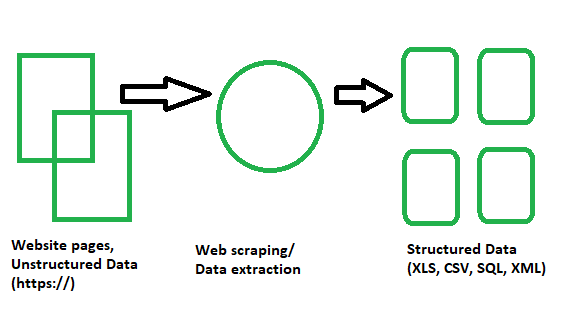
\includegraphics[width=0.5\textwidth]{./pics/web.png}
    \caption{Gathering data from webpages}
    \label{fig:webpages}
\end{figure}

As our first step, we are going to use Python \textbf{requests} library to get a web page data as HTML format.
The Python \textbf{requests}  library is a powerful library for making HTTP requests in Python.
It simplifies the process of sending HTTP requests and receiving responses, making it easy to interact with web services and APIs (application programming interface).

Here's a simple example of how to make a GET request using the \textbf{requests} library:

\begin{lstlisting}[language=Python, caption=Example of getting a page content]
import requests

# fetching data from a Wikipedia page
response = requests.get("https://en.wikipedia.org/wiki/Helium")

# using response object to get the fetched details
print(response.status_code)
print(response.text)
print(response.content)
\end{lstlisting}

In the code above, we openend a link and extracted its content as a string.
Now I want you to use this example in order to get an input link and extract its content into a string variable.

\begin{warning}
Remember that if the input link is incorrent or returns an error, your Python code may crash.
Therefore, make sure to handle these types of errors by using page \underline{status code} field and Python try/exept feature.
\end{warning}

\subsection{Scraping Page Content}
Python has several libraries to scrape web pages. Let's see the web scraping libraries in Python:

\begin{itemize}
    \item Requests (HTTP for Humans) Library for Web Scraping: It is used for making various types of HTTP requests like GET, POST, etc. It is the most basic yet the most essential of all libraries.
    \item lxml Library for Web Scraping: lxml library provides super-fast and high-performance parsing of HTML and XML content from websites. If you are planning to scrape large datasets, this is the one you should go for.
    \item Beautiful Soup Library for Web Scraping: Its work involves creating a parse tree for parsing content. A perfect starting library for beginners and very easy to work with.
    \item Selenium Library for Web Scraping: Originally made for automated testing of web applications, this library overcomes the issue all the above libraries face i.e. scraping content from dynamically populated websites. This makes it slower and not suitable for industry-level projects.
    \item Scrapy for Web Scraping: The BOSS of all libraries, an entire web scraping framework which is asynchronous in its usage. This makes it blazing fast and increases efficiency.
\end{itemize}

Now we are going to use Python beautiful soup library in order to parse HTML content in to a list of paragraphs.

\begin{lstlisting}[language=Python, caption=Example of using BS4 library]
# import required modules
from bs4 import BeautifulSoup

# scrape webpage
soup = BeautifulSoup(response.content, 'html.parser')
 
# find all occurrence of p in HTML
# includes HTML tags
print(soup.find_all('p'))
\end{lstlisting}

The example above gets all `p` tags that are paragraphs in a HTML page. Now I want you to migrate
this example with your previous code in order to extract all paragraphs' contents from a Wikipedia page
and save them into a text file.

\subsection{Creating Index Table}
In this section we are going to analyze our contents in order to categorize our Wikipedia pages. In order to do this,
we are using a concept in Information Retrieval called Inverted Index.

An Inverted Index is a data structure used in information retrieval systems to efficiently retrieve documents or web pages
containing a specific term or set of terms.
In an inverted index, the index is organized by terms (words), and each term points to a list of documents or web pages that contain that term.

Generally there are three steps in building an inverted index:
\begin{enumerate}
    \item Fetch the Document: Removing of Stop Words: Stop words are the most occurring and useless words in documents like "I", "the", "we", "is", and "an".
    \item Stemming of Root Word: Whenever I want to search for "cat", I want to see a document that has information about it. But the word present in the document is called "cats" or "catty" instead of "cat". To relate both words, I'll chop some part of every word I read so that I could get the "root word". There are standard tools for performing this like "Porter's Stemmer".
    \item Record Document IDs: If the word is already present add a reference of the document to index else creates a new entry. Add additional information like the frequency of the word, location of the word, etc.
\end{enumerate}

In Figure~\ref{fig:invertindex} you can see the process of creating an inverted index from one or more documents.

\begin{figure}[h]
    \centering
    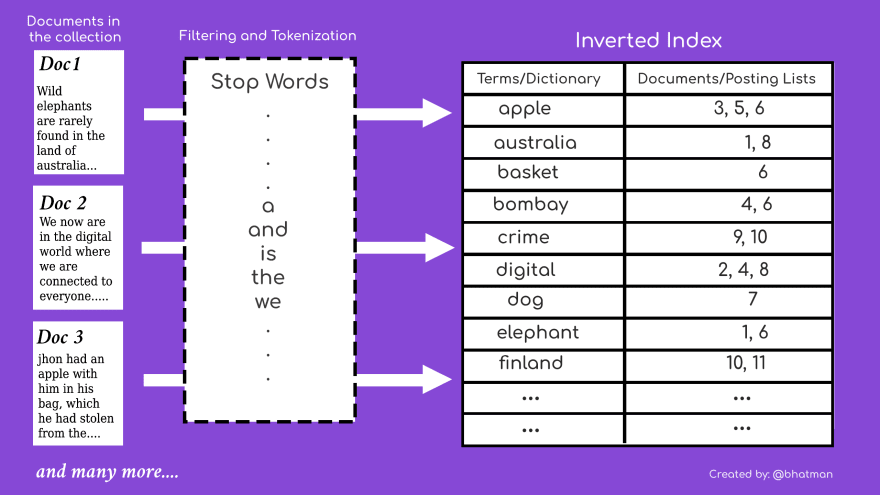
\includegraphics[width=0.8\textwidth]{./pics/invert-index.png}
    \caption{Inverted Index}
    \label{fig:invertindex}
\end{figure}

Now I want you to read the text files from previous section, and create an inverted index for each of them. You don't need
to merge all files; just create an inverted index for each Wikipedia page content. Finally, with an inverted index you can categorize your documents by analyzing the most words in their text. Make sure to
suggest at least three categories for each Wikipedia page.

\begin{suggestion}
There are some most used english words like `is`, `the`, etc. which are used alot in a paragraph. These words cannot be returned
as a page categories since they are not an entity. Search through the internet to find how you can fix this issue.
\end{suggestion}

\section{Expected Outcomes}
We anticipate achieving the following outcomes:
\begin{itemize}
    \item Successful extraction of data from Wikipedia pages using \textbf{requests} module.
    \item Accurate determination of page titles based on content analysis using \textbf{beautiful soup}.
    \item Contribution to the understanding of web scraping and information retrieval inverted index technique.
\end{itemize}

\section{References}
\begin{itemize}
    \item \href{https://www.geeksforgeeks.org/inverted-index/}{geeksforgeeks.org/inverted-index}
    \item \href{https://www.geeksforgeeks.org/web-scraping-from-wikipedia-using-python-a-complete-guide/}{geeksforgeeks.org/web-scraping}
\end{itemize}

\end{document}
